\begin{figure*}[hbtp]
  \centering
  \subfigure[Runtime in seconds (logarithmic scale) for link prediction using the best similarity measure, with \textit{IBase} and \textit{DLH} approaches]{
    \label{fig:input-large--runtime}
    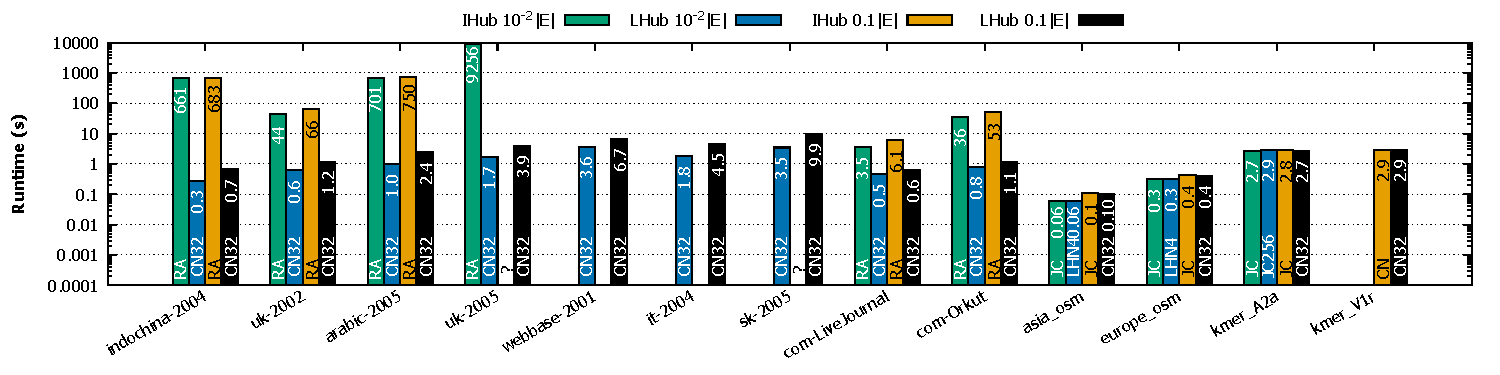
\includegraphics[width=0.98\linewidth]{out/input-large-runtime.pdf}
  }
  \subfigure[Speedup (logarithmic scale) for link prediction with the best similarity measure of \textit{DLH} approach, compared to \textit{IBase} approach]{
    \label{fig:input-large--speedup}
    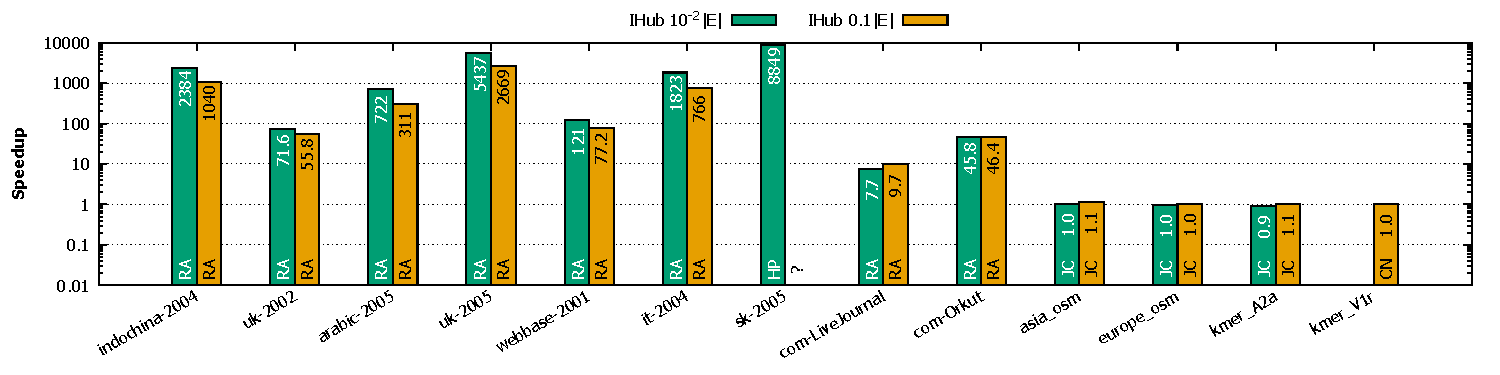
\includegraphics[width=0.98\linewidth]{out/input-large-speedup.pdf}
  }
  \subfigure[F1 score of predicted links (logarithmic scale), for link prediction using the best similarity measure, with \textit{IBase} and \textit{DLH} approaches]{
    \label{fig:input-large--f1score}
    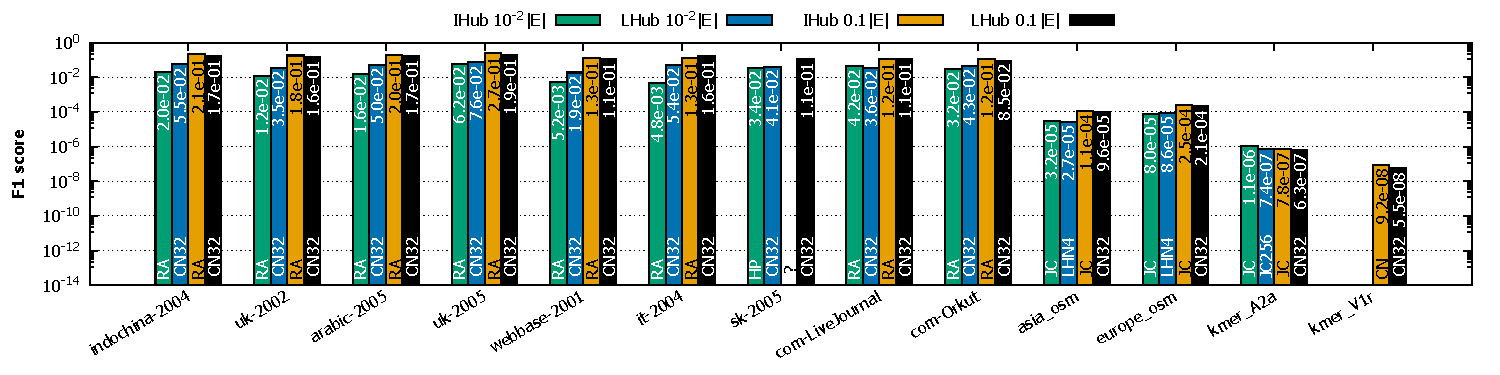
\includegraphics[width=0.98\linewidth]{out/input-large-f1score.pdf}
  } \\[-2ex]
  \caption{Runtime in seconds (log-scale), speedup (log-scale), and F1 score of predicted links (log-scale), for link prediction with the \textit{Improved Baseline (IBase)} approach and our approach of \textit{Disregarding Large Hubs (DLH)}, using the best similarity measure, when attempting to predict $10^{-2}|E|$ to $0.1|E|$ unobserved edges $E^U$, for each graph\ignore{in the dataset}. For each similarity measure outlined in Section \ref{sec:metrics}, we attempt only the best hub limit $L_H$ parameter setting obtained in Section \ref{sec:select-limit} (for the \textit{DLH} approach), and then select the best among them, considering both the F1 score and runtime. Note that the numerical suffix added to the acronym of each link prediction method, with the \textit{DLH} approach, indicates the hub limit $L_H$ parameter setting.}
  \label{fig:input-large}
\end{figure*}
